% ============================================================
%  Real-Time Crime Analytics — Project Report
%  Big Data Analytics, FAST NUCES Islamabad
%  Compile with: pdflatex → bibtex → pdflatex × 2
%  (or just pdflatex twice on Overleaf — no bibliography needed)
% ============================================================
\documentclass[11pt,a4paper]{article}

% ── Packages ──────────────────────────────────────────────
\usepackage[margin=2cm,top=2.2cm,bottom=2.2cm]{geometry}
\usepackage[T1]{fontenc}
\usepackage{lmodern}
\usepackage{microtype}
\usepackage{graphicx}
\usepackage{booktabs}
\usepackage{array}
\usepackage{longtable}
\usepackage{xcolor}
\usepackage{colortbl}
\usepackage{tikz}
\usepackage{pgfplots}
\pgfplotsset{compat=1.18}
\usetikzlibrary{positioning,arrows.meta,shapes,fit,backgrounds,calc}
\usepackage{hyperref}
\usepackage{enumitem}
\usepackage{fancyhdr}
\usepackage{titlesec}
\usepackage{amsmath}
\usepackage{caption}
\usepackage{subcaption}
\usepackage{float}
\usepackage{listings}
\usepackage{parskip}

% ── Colours ───────────────────────────────────────────────
\definecolor{primary}{RGB}{0,84,166}
\definecolor{secondary}{RGB}{220,38,38}
\definecolor{accent}{RGB}{5,150,105}
\definecolor{lightgray}{RGB}{245,245,245}
\definecolor{darkgray}{RGB}{60,60,60}
\definecolor{batchcol}{RGB}{59,130,246}
\definecolor{speedcol}{RGB}{239,68,68}
\definecolor{servcol}{RGB}{16,185,129}

% ── Section formatting ────────────────────────────────────
\titleformat{\section}{\large\bfseries\color{primary}}{}{0em}{\thesection\enspace}[\titlerule]
\titleformat{\subsection}{\normalsize\bfseries\color{darkgray}}{}{0em}{\thesubsection\enspace}
\titleformat{\subsubsection}{\normalsize\itshape\color{darkgray}}{}{0em}{\thesubsubsection\enspace}

% ── Header / Footer ───────────────────────────────────────
\pagestyle{fancy}
\fancyhf{}
\fancyhead[L]{\small\color{darkgray}Real-Time Crime Analytics — Big Data Project}
\fancyhead[R]{\small\color{darkgray}FAST NUCES, Islamabad}
\fancyhead[R]{\small\color{darkgray}Atif Ibrahim Abbasi,i22-1249 }
\fancyhead[R]{\small\color{darkgray}M. Ali ,22i-0827 }
\fancyfoot[C]{\small\thepage}
\renewcommand{\headrulewidth}{0.4pt}

% ── Listings style ────────────────────────────────────────
\lstset{
  basicstyle=\ttfamily\footnotesize,
  backgroundcolor=\color{lightgray},
  frame=single,
  breaklines=true,
  columns=fullflexible
}

% ── Hyperref colours ──────────────────────────────────────
\hypersetup{colorlinks=true,linkcolor=primary,urlcolor=accent}

% ── Table helpers ─────────────────────────────────────────
\newcolumntype{L}[1]{>{\raggedright\arraybackslash}p{#1}}
\newcolumntype{C}[1]{>{\centering\arraybackslash}p{#1}}
\newcolumntype{R}[1]{>{\raggedleft\arraybackslash}p{#1}}

% ──────────────────────────────────────────────────────────
%  TITLE PAGE
% ──────────────────────────────────────────────────────────
\begin{document}

\begin{titlepage}
\centering
\vspace*{1.5cm}

{\color{primary}\rule{\linewidth}{2pt}}
\vspace{0.5cm}

{\Huge\bfseries Real-Time Crime Analytics\\[0.4em]
\large\normalfont Using Lambda Architecture on Chicago Crime Data}

\vspace{0.4cm}
{\color{primary}\rule{\linewidth}{0.6pt}}

\vspace{1.2cm}


\begin{tikzpicture}
  \node[draw=primary,fill=primary!8,rounded corners=8pt,
        inner sep=14pt,text width=10cm,align=center] {
    \textbf{Big Data Analytics — Project Report}\\[4pt]
    FAST National University of Computer and Emerging Sciences\\
    Islamabad Campus\\[8pt]
    \textit{Course: Big Data Analytics}\\
    \textit{Author: Muhammad Ali \quad (i220827)}\\[4pt]
    \textit{Author: Atif Ibrahim Abbasi \quad (i22-1249)}\\[4pt]
   
    \textit{Date: May 2026}
  };
\end{tikzpicture}

\vspace{1.4cm}

\begin{abstract}
\noindent
This report presents the design, implementation, and analytical results of a
\textbf{Lambda Architecture} system for real-time and batch analysis of Chicago
crime data. The system ingests 50{,}000 crime incident records alongside
10{,}000 arrest records, 10{,}000 violence reduction records, 10{,}000 sex
offender records, and all Chicago police stations. Apache Spark handles the
batch layer (preprocessing, business intelligence, and machine learning), a
Kafka-Storm pipeline constitutes the speed layer for real-time anomaly
detection, and PostgreSQL/MongoDB form the serving layer consumed by a
Streamlit dashboard. Key findings include identification of ten geospatial
crime hotspots via KMeans clustering, peak crime hours at midnight and
mid-afternoon, a 97.4\% gunshot injury proportion in violence incidents, and
2{,}264 real-time anomaly alerts generated during simulation. Challenges with
data heterogeneity, distributed coordination, and schema evolution are
discussed alongside mitigation strategies.
\end{abstract}

\vspace{0.8cm}
{\color{primary}\rule{\linewidth}{2pt}}
\end{titlepage}

\tableofcontents
\newpage

% ──────────────────────────────────────────────────────────
%  1. INTRODUCTION
% ──────────────────────────────────────────────────────────
\section{Introduction}

Urban crime analysis has increasingly benefited from the application of
big data techniques, enabling law enforcement agencies to move from
reactive to predictive policing strategies. Traditional relational
databases and batch-oriented ETL pipelines cannot satisfy the dual demand
for (a)~historical, high-accuracy analytical queries and (b)~near-real-time
situational awareness when crime events are in progress.

This project implements a \textbf{Lambda Architecture} on five openly
available Chicago datasets to demonstrate that a modern big data stack
can address both demands simultaneously. The architecture decomposes the
problem into three layers:

\begin{itemize}[noitemsep]
  \item \textbf{Batch Layer} — Apache Spark computes immutable, accurate
    analytics over the full historical dataset on a periodic cadence.
  \item \textbf{Speed Layer} — Apache Kafka streams live crime events to a
    Storm-style Python topology that detects anomalies within a 5-minute
    sliding window.
  \item \textbf{Serving Layer} — PostgreSQL and MongoDB store precomputed
    views and real-time alerts, respectively, for fast dashboard queries.
\end{itemize}

The remainder of this report is structured as follows:
Section~2 describes the system architecture;
Section~3 covers the data schema;
Section~4 details the analytics methodology;
Section~5 describes the machine learning approach;
Section~6 presents experimental results;
Section~7 discusses challenges and mitigations.

% ──────────────────────────────────────────────────────────
%  2. SYSTEM DESIGN
% ──────────────────────────────────────────────────────────
\section{System Design}

\subsection{Lambda Architecture Overview}

The Lambda Architecture, proposed by Nathan Marz, separates data
processing into three complementary layers. Figure~\ref{fig:arch} shows
the high-level topology used in this project.

\begin{figure}[H]
\centering
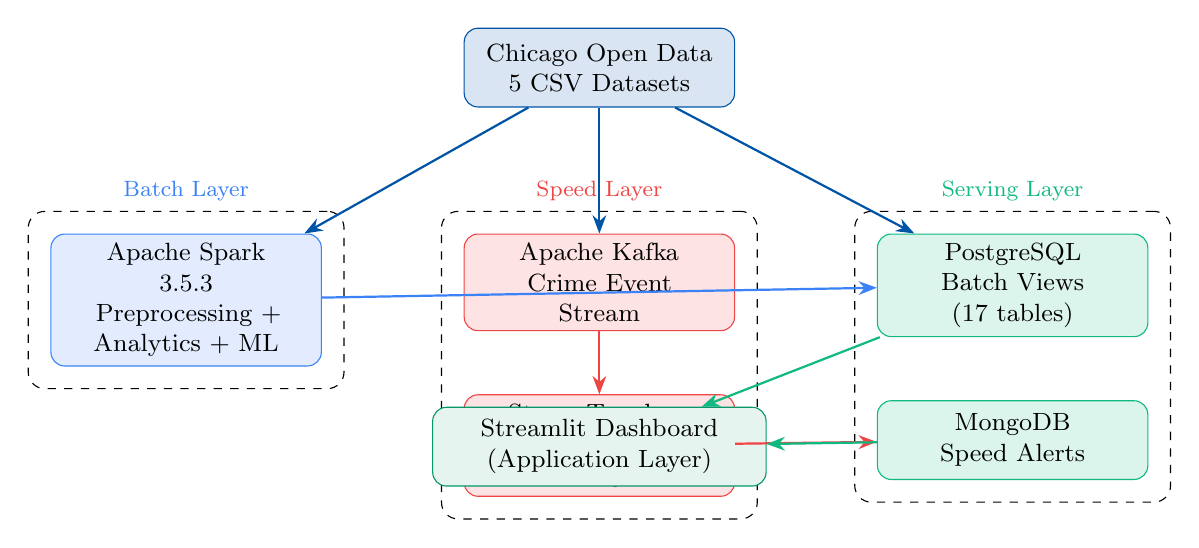
\begin{tikzpicture}[
  box/.style={draw,rounded corners=5pt,minimum height=1cm,
              text width=3.2cm,align=center,font=\small},
  layer/.style={draw,dashed,rounded corners=6pt,inner sep=8pt},
  arr/.style={-{Stealth},thick}
]

% Data source
\node[box,fill=primary!15,draw=primary] (src) {Chicago Open Data\\5 CSV Datasets};

% Batch layer
\node[box,fill=batchcol!15,draw=batchcol,below left=1.6cm and 1.8cm of src] (spark) {Apache Spark\\3.5.3\\Preprocessing +\\Analytics + ML};

% Speed layer
\node[box,fill=speedcol!15,draw=speedcol,below=1.6cm of src] (kafka) {Apache Kafka\\Crime Event\\Stream};
\node[box,fill=speedcol!15,draw=speedcol,below=0.8cm of kafka] (storm) {Storm Topology\\ParseBolt $\to$\\AnomalyBolt};

% Serving layer
\node[box,fill=servcol!15,draw=servcol,below right=1.6cm and 1.8cm of src] (pg) {PostgreSQL\\Batch Views\\(17 tables)};
\node[box,fill=servcol!15,draw=servcol,below=0.8cm of pg] (mongo) {MongoDB\\Speed Alerts};

% App layer
\node[box,fill=accent!10,draw=accent,below=3.8cm of src,text width=4cm] (dash) {Streamlit Dashboard\\(Application Layer)};

% Arrows
\draw[arr,primary] (src) -- (spark);
\draw[arr,primary] (src) -- (kafka);
\draw[arr,primary] (src) -- (pg);
\draw[arr,speedcol] (kafka) -- (storm);
\draw[arr,batchcol] (spark) -- (pg);
\draw[arr,speedcol] (storm) -- (mongo);
\draw[arr,servcol] (pg) -- (dash);
\draw[arr,servcol] (mongo) -- (dash);

% Layer brackets
\begin{pgfonlayer}{background}
  \node[layer,fit=(spark),label=above:{\color{batchcol}\footnotesize Batch Layer}] {};
  \node[layer,fit=(kafka)(storm),label=above:{\color{speedcol}\footnotesize Speed Layer}] {};
  \node[layer,fit=(pg)(mongo),label=above:{\color{servcol}\footnotesize Serving Layer}] {};
\end{pgfonlayer}
\end{tikzpicture}
\caption{High-level Lambda Architecture for the Real-Time Crime Analytics system.}
\label{fig:arch}
\end{figure}

\subsection{Component Details}

\subsubsection{Batch Layer — Apache Spark}
Spark 3.5.3 is deployed in master-worker mode via Docker Compose with
2 GB RAM and 2 cores allocated to the worker. Five preprocessing jobs
convert raw CSV files to Parquet with explicit schemas, after which
five analytics jobs compute business intelligence views and one ML job
runs KMeans clustering. All results are persisted to PostgreSQL via the
JDBC connector (\texttt{postgresql-42.7.3.jar}).

\subsubsection{Speed Layer — Kafka + Storm Topology}
Apache Kafka (backed by Zookeeper) exposes a single topic
\texttt{crime\_events}. A Kafka producer simulates a live crime feed by
reading rows from \texttt{crimes.csv} at 5 events/second. The Storm-style
Python topology consumes the topic and chains six processing stages:

\begin{center}
\ttfamily\small
KafkaSpout $\to$ ParseBolt $\to$ DistrictBolt $\to$ WindowBolt $\to$ AnomalyBolt $\to$ AlertBolt
\end{center}

The \textbf{WindowBolt} maintains a per-district deque of timestamps,
pruning events older than 300 seconds. The \textbf{AnomalyBolt} fires an
alert when the window count exceeds a configurable threshold (default: 5)
and assigns a severity (CRITICAL $\geq$ 3$\times$, HIGH $\geq$ 2$\times$,
MEDIUM $\geq$ 1.5$\times$, LOW otherwise).

\subsubsection{Serving Layer — PostgreSQL and MongoDB}
PostgreSQL~15 stores 20 precomputed analytical tables accessed by the
Streamlit dashboard via SQL. MongoDB~6.0 acts as a document store for
speed-layer alert logs, enabling flexible schema evolution and fast
append writes during peak anomaly activity.

\subsubsection{Application Layer — Streamlit}
A Streamlit dashboard (port 8501) provides interactive visualisations
for both batch views and live alerts, querying PostgreSQL for historical
analytics and MongoDB for the real-time alert feed.

\subsection{Infrastructure}
All nine services are orchestrated by Docker Compose on a single bridge
network (\texttt{lambda\_net}). Table~\ref{tab:services} lists every
service, its base image, and exposed port.

\begin{table}[H]
\centering
\caption{Docker Compose service inventory.}
\label{tab:services}
\begin{tabular}{@{}llcl@{}}
\toprule
\textbf{Container} & \textbf{Image} & \textbf{Port} & \textbf{Role} \\
\midrule
\texttt{zookeeper}    & wurstmeister/zookeeper  & 2181 & Kafka coordination \\
\texttt{kafka}        & wurstmeister/kafka      & 9092 & Stream broker \\
\texttt{nimbus}       & storm:2.5.0             & 6627 & Storm Nimbus \\
\texttt{supervisor}   & storm:2.5.0             & —    & Storm worker \\
\texttt{storm-ui}     & storm:2.5.0             & 8080 & Storm Web UI \\
\texttt{spark-master} & apache/spark:3.5.3      & 7077,\,8081 & Spark Master \\
\texttt{spark-worker} & apache/spark:3.5.3      & —    & Spark executor \\
\texttt{postgres}     & postgres:15-alpine      & 5432 & Serving DB (SQL) \\
\texttt{mongodb}      & mongo:6.0               & 27017 & Serving DB (NoSQL) \\
\texttt{streamlit}    & python:3.9-slim-buster  & 8501 & Dashboard \\
\bottomrule
\end{tabular}
\end{table}

% ──────────────────────────────────────────────────────────
%  3. DATA SCHEMA
% ──────────────────────────────────────────────────────────
\section{Data Schema}

\subsection{Source Datasets}

Five datasets are ingested from the Chicago Open Data Portal:

\begin{table}[H]
\centering
\caption{Source dataset summary.}
\label{tab:sources}
\begin{tabular}{@{}llr@{}}
\toprule
\textbf{File} & \textbf{Description} & \textbf{Records} \\
\midrule
\texttt{crimes.csv}          & Crime incidents (IUCR-coded) & 50{,}000 \\
\texttt{arrests.csv}         & Arrest records with demographics & 10{,}000 \\
\texttt{violence.csv}        & CPD violence reduction incidents & 10{,}000 \\
\texttt{sex\_offenders.csv}  & Registered sex offender locations & 10{,}000 \\
\texttt{police\_stations.csv} & Station locations \& districts & 22 \\
\bottomrule
\end{tabular}
\end{table}

\subsection{PostgreSQL Serving Schema}

After Spark batch processing and the speed-layer pipeline, 20 tables are
materialised in PostgreSQL. They fall into four logical groups:

\begin{longtable}{@{}L{4.6cm}L{1.8cm}L{7cm}@{}}
\caption{PostgreSQL serving-layer tables.}\label{tab:schema}\\
\toprule
\textbf{Table} & \textbf{Source} & \textbf{Description} \\
\midrule
\endfirsthead
\toprule
\textbf{Table} & \textbf{Source} & \textbf{Description} \\
\midrule
\endhead
\midrule\multicolumn{3}{r}{\small\itshape Continued on next page}
\endfoot
\bottomrule
\endlastfoot

\multicolumn{3}{@{}l}{\small\itshape\color{batchcol}Crime Trend Tables} \\
\texttt{crime\_trends\_by\_year}         & Batch & Crime count aggregated by calendar year \\
\texttt{crime\_trends\_by\_month}        & Batch & Crime count by year and month \\
\texttt{crime\_trends\_by\_day\_of\_week} & Batch & Crime count per day of week (1=Sun, 7=Sat) \\
\texttt{crime\_trends\_by\_hour}         & Batch & Crime count per hour of day (0–23) \\
\addlinespace
\multicolumn{3}{@{}l}{\small\itshape\color{batchcol}Arrest Analysis Tables} \\
\texttt{arrest\_rate\_by\_crime\_type}   & Batch & Arrest rate per IUCR primary type \\
\texttt{top10\_crime\_types\_by\_arrest\_rate} & Batch & Top-10 crime types ranked by arrest rate \\
\texttt{arrest\_rate\_by\_district}      & Batch & Per-district arrest rate \\
\texttt{arrests\_by\_race}               & Batch & Arrestee counts stratified by race \\
\addlinespace
\multicolumn{3}{@{}l}{\small\itshape\color{batchcol}Violence \& Gunshot Tables} \\
\texttt{violence\_by\_month}             & Batch & Homicide vs.\ non-fatal incidents by month \\
\texttt{violence\_by\_district}          & Batch & Violence incident counts per district \\
\texttt{gunshot\_injury\_proportion}     & Batch & Overall gunshot injury rate (global) \\
\texttt{gunshot\_proportion\_by\_district} & Batch & Gunshot injury rate per police district \\
\texttt{top\_community\_areas\_by\_violence} & Batch & Community areas ranked by total violence \\
\addlinespace
\multicolumn{3}{@{}l}{\small\itshape\color{batchcol}Offender \& Correlation Tables} \\
\texttt{sex\_offender\_density\_by\_district} & Batch & Registered offenders per district \\
\texttt{sex\_offenders\_minor\_victims\_priority} & Batch & Offenders with minor victim flag \\
\texttt{district\_arrest\_vs\_violence\_correlation} & Batch & Per-district arrest rate vs.\ violence rate \\
\texttt{community\_offender\_vs\_crime\_correlation} & Batch & Community-level offender density vs.\ crime rate \\
\addlinespace
\multicolumn{3}{@{}l}{\small\itshape\color{batchcol}ML Output Tables} \\
\texttt{hotspots}                        & ML    & KMeans cluster centroids (k=10) with crime counts \\
\texttt{crimes\_with\_clusters}          & ML    & Each crime record labelled with cluster ID \\
\addlinespace
\multicolumn{3}{@{}l}{\small\itshape\color{speedcol}Speed Layer Table} \\
\texttt{speed\_layer\_alerts}            & Speed & Real-time anomaly alerts with severity and location \\
\end{longtable}

\subsection{Key Table Definitions}

\paragraph{speed\_layer\_alerts} Contains columns \texttt{alert\_id} (VARCHAR),
\texttt{alert\_type}, \texttt{district}, \texttt{crime\_count\_in\_window}
(INT), \texttt{window\_seconds} (INT), \texttt{threshold} (INT),
\texttt{latest\_crime\_type}, \texttt{latitude}/\texttt{longitude} (DOUBLE),
\texttt{triggered\_at} (TIMESTAMP), and \texttt{severity}. Indexed on
\texttt{district}, \texttt{severity}, and \texttt{triggered\_at} for fast
dashboard filter queries.

\paragraph{hotspots} Contains \texttt{cluster\_id} (INT),
\texttt{centroid\_latitude}, \texttt{centroid\_longitude} (DOUBLE), and
\texttt{crime\_count} (INT) representing the number of crimes assigned to
each cluster centre.

% ──────────────────────────────────────────────────────────
%  4. ANALYTICS METHODOLOGY
% ──────────────────────────────────────────────────────────
\section{Analytics Methodology}

\subsection{Batch Analytics Pipeline (Spark)}

The batch layer is implemented as a single PySpark job
(\texttt{batch\_analytics.py}) comprising five analytical modules executed
sequentially on preprocessed Parquet files.

\subsubsection{Data Preprocessing}
Raw CSVs are ingested with \emph{explicit} schemas (no \texttt{inferSchema})
to ensure deterministic column types across Spark workers. Timestamp
columns are parsed with \texttt{to\_timestamp}, categorical columns are
trimmed of whitespace, and invalid latitude/longitude values are filtered
out. Clean data is written to Parquet (columnar, compressed) in
\texttt{/data/cleaned/} for optimal Spark scan performance.

\subsubsection{Crime Trend Analysis (§7.1)}
Temporal components are extracted from the \texttt{date} column using
Spark's \texttt{year()}, \texttt{month()}, \texttt{dayofweek()}, and
\texttt{hour()} functions. Four aggregation tables capture crime volume
at different temporal granularities:

\begin{equation}
\text{CrimeCount}(g) = \sum_{i=1}^{N} \mathbf{1}[\text{date}_i \in g]
\end{equation}

where $g$ is a temporal grouping (year, month, day-of-week, or hour).

\subsubsection{Arrest Rate Analysis (§7.2)}
Crimes and arrests are joined on \texttt{case\_number} (left join) to
flag which incidents resulted in an arrest. Arrest rate per category is:

\begin{equation}
\text{ArrestRate}(c) = \frac{\text{Arrests in category } c}{\text{Crimes in category } c}
\end{equation}

This is computed for primary crime type, police district, and arrestee
race. A minimum crime count of 10 is enforced before a type qualifies
for the top-10 ranking to avoid statistical noise from rare offences.

\subsubsection{Violence and Gunshot Analysis (§7.3)}
The violence dataset records each incident with a
\texttt{victimization\_primary} label (\textsc{battery}, \textsc{homicide},
\textsc{robbery}, etc.) and a binary \texttt{gunshot\_injury\_i} flag.
Monthly and district-level breakdowns are computed via \texttt{groupBy}
aggregations. The overall gunshot proportion is:

\begin{equation}
P(\text{gunshot}) = \frac{\sum_{i=1}^{N} \mathbf{1}[\texttt{gunshot\_injury\_i}_i = \text{YES}]}{N}
\end{equation}

\subsubsection{Sex Offender Proximity Analysis (§7.4)}
Sex offenders are not directly tagged with a police district. A
block$\to$district lookup is derived from the crimes dataset using a
window function that selects the most frequent district per block.
Offenders are mapped to districts via this lookup and counted. Priority
records with \texttt{victim\_minor = Y} are extracted into a separate
table for rapid law enforcement access.

\subsubsection{Cross-Dataset Correlation (§7.6)}
Two cross-dataset correlations are computed:
\begin{enumerate}[noitemsep]
  \item \textbf{Arrest rate vs.\ violence rate per district} — crimes,
    arrests, and violence tables are joined on \texttt{district}.
  \item \textbf{Sex offender density vs.\ crime rate per community area}
    — sex offenders are mapped to community areas via the block lookup,
    then joined with community-level crime counts.
\end{enumerate}

\subsection{Speed Layer — Storm Topology}

The speed layer implements a Python-based streaming topology with six
stages, each encapsulated in a bolt class.

\begin{table}[H]
\centering
\caption{Storm topology bolt responsibilities.}
\label{tab:bolts}
\begin{tabular}{@{}llL{7.5cm}@{}}
\toprule
\textbf{Stage} & \textbf{Component} & \textbf{Responsibility} \\
\midrule
1 & KafkaSpout      & Polls \texttt{crime\_events} Kafka topic; emits raw JSON strings. \\
2 & ParseBolt       & Validates and deserialises JSON; discards malformed messages. \\
3 & DistrictBolt    & Routes events by \texttt{district} field; tracks active districts. \\
4 & WindowBolt      & Maintains per-district deque; prunes events $>$ 300 s old; annotates with \texttt{window\_count}. \\
5 & AnomalyBolt     & Compares \texttt{window\_count} to threshold; assigns severity; emits alert dict. \\
6 & AlertBolt       & Persists alert to PostgreSQL (\texttt{speed\_layer\_alerts}) and MongoDB (\texttt{alert\_logs}). \\
\bottomrule
\end{tabular}
\end{table}

% ──────────────────────────────────────────────────────────
%  5. ML APPROACH
% ──────────────────────────────────────────────────────────
\section{Machine Learning Approach}

\subsection{Objective}
The goal of the ML component (§7.5) is to identify geospatial crime
hotspots — compact geographic clusters with disproportionately high
crime volumes — to guide patrol resource allocation.

\subsection{Algorithm: KMeans Clustering}
PySpark MLlib's \texttt{KMeans} algorithm is applied to the crime
dataset filtered to records with valid latitude and longitude
(approximately 49{,}800 records out of 50{,}000). The feature vector is:

\begin{equation}
\mathbf{x}_i = [\text{latitude}_i,\; \text{longitude}_i]^{\top}
\end{equation}

Hyperparameters are set to $k=10$ clusters, \texttt{seed=42} for
reproducibility, and default Euclidean distance. Model quality is
evaluated using Within-Set Sum of Squared Errors (WSSSE):

\begin{equation}
\text{WSSSE} = \sum_{k=1}^{K} \sum_{\mathbf{x} \in C_k}
  \left\| \mathbf{x} - \boldsymbol{\mu}_k \right\|^2
\end{equation}

where $\boldsymbol{\mu}_k$ is the centroid of cluster $C_k$.

\subsection{Implementation Workflow}

\begin{enumerate}[noitemsep]
  \item Load \texttt{crimes.parquet}; filter null geo-coordinates.
  \item Assemble \texttt{[latitude, longitude]} into a feature vector
    using \texttt{VectorAssembler}.
  \item Train \texttt{KMeans(k=10, seed=42)}.
  \item Extract cluster centroids and join with per-cluster crime counts.
  \item Persist centroid table (\texttt{hotspots}) and labelled crimes
    (\texttt{crimes\_with\_clusters}) to PostgreSQL.
\end{enumerate}

\subsection{Rationale for KMeans}

KMeans was selected over DBSCAN or hierarchical clustering for three
reasons:
(1) it scales linearly with the number of records on Spark's distributed
MLlib;
(2) a fixed $k$ is operationally convenient (one patrol zone per cluster);
(3) the relatively uniform geographic spread of Chicago crime incidents
does not exhibit strong non-convex cluster shapes that would require
density-based methods.

% ──────────────────────────────────────────────────────────
%  6. RESULTS
% ──────────────────────────────────────────────────────────
\section{Results}

\subsection{Crime Temporal Patterns}

\subsubsection{Crimes by Hour of Day}

\begin{figure}[H]
\centering
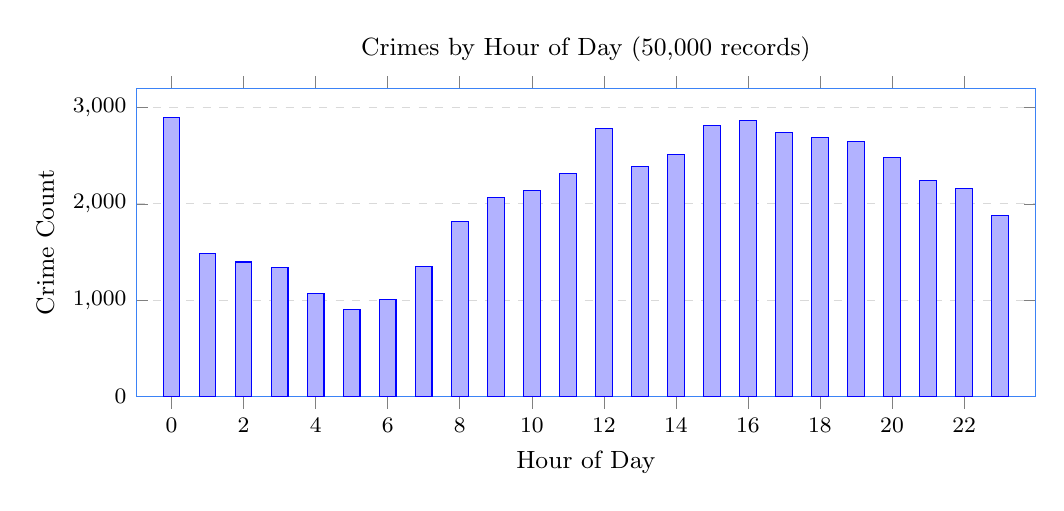
\begin{tikzpicture}
\begin{axis}[
  width=13cm, height=5.5cm,
  ybar, bar width=6pt,
  xlabel={Hour of Day}, ylabel={Crime Count},
  xtick={0,2,4,6,8,10,12,14,16,18,20,22},
  xticklabels={0,2,4,6,8,10,12,14,16,18,20,22},
  xmin=-0.5, xmax=23.5,
  ymin=0, ymax=3200,
  ymajorgrids=true, grid style={dashed,gray!30},
  bar shift=0pt,
  fill=batchcol!70, draw=batchcol,
  title={\small Crimes by Hour of Day (50{,}000 records)},
  title style={font=\small},
  tick label style={font=\footnotesize},
  label style={font=\small},
  enlarge x limits=0.02
]
\addplot coordinates {
  (0,2897)(1,1482)(2,1397)(3,1342)(4,1069)(5,904)
  (6,1011)(7,1353)(8,1820)(9,2068)(10,2141)(11,2313)
  (12,2784)(13,2384)(14,2515)(15,2810)(16,2863)(17,2740)
  (18,2691)(19,2643)(20,2485)(21,2243)(22,2163)(23,1882)
};
\end{axis}
\end{tikzpicture}
\caption{Crime volume peaks at midnight (hour 0: 2{,}897), 15:00–16:00 (2{,}863), and 12:00 (2{,}784). The lowest activity is at 05:00 (904 crimes).}
\label{fig:hour}
\end{figure}

\subsubsection{Crimes by Day of Week}

\begin{figure}[H]
\centering
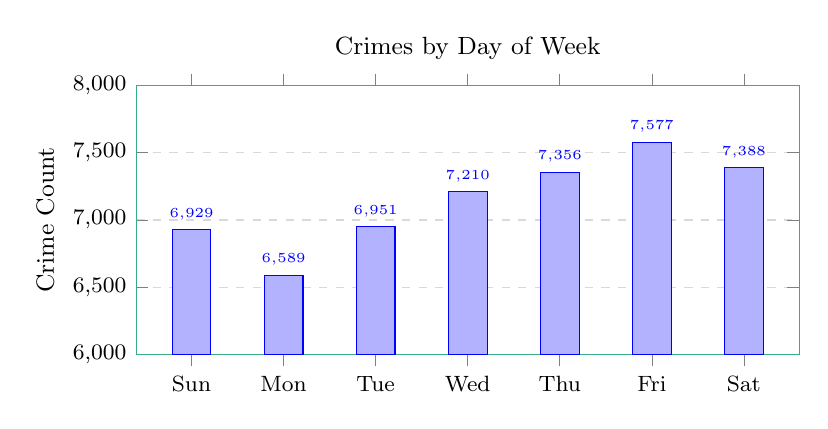
\begin{tikzpicture}
\begin{axis}[
  width=10cm, height=5cm,
  ybar, bar width=14pt,
  symbolic x coords={Sun,Mon,Tue,Wed,Thu,Fri,Sat},
  xtick=data,
  ylabel={Crime Count},
  ymin=6000, ymax=8000,
  ymajorgrids=true, grid style={dashed,gray!30},
  fill=accent!60, draw=accent!80,
  title={\small Crimes by Day of Week},
  title style={font=\small},
  tick label style={font=\footnotesize},
  label style={font=\small},
  nodes near coords,
  nodes near coords style={font=\tiny,above}
]
\addplot coordinates {
  (Sun,6929)(Mon,6589)(Tue,6951)(Wed,7210)(Thu,7356)(Fri,7577)(Sat,7388)
};
\end{axis}
\end{tikzpicture}
\caption{Friday records the highest crime volume (7{,}577), with Monday the lowest (6{,}589). The mid-week through weekend trend suggests increased activity as the week progresses.}
\label{fig:dow}
\end{figure}

\subsection{Arrest Rate Analysis}

\begin{table}[H]
\centering
\caption{Top-10 crime types by arrest rate (minimum 10 incidents).}
\label{tab:arrest}
\begin{tabular}{@{}L{7cm}rrl@{}}
\toprule
\textbf{Crime Type} & \textbf{Total Crimes} & \textbf{Arrests} & \textbf{Arrest Rate} \\
\midrule
Concealed Carry License Violation &  46 &  37 & \textbf{80.4\%} \\
Prostitution                       &  42 &  29 & 69.1\% \\
Interference with Public Officer   & 220 & 144 & 65.5\% \\
Weapons Violation                  &1{,}095 & 655 & 59.8\% \\
Narcotics                          &1{,}587 & 936 & 59.0\% \\
Public Peace Violation             & 263 &  93 & 35.4\% \\
Criminal Trespass                  &1{,}243 & 377 & 30.3\% \\
Homicide                           &  99 &  18 & 18.2\% \\
Battery                            &9{,}279 &1{,}520 & 16.4\% \\
Other Offense                      &3{,}554 & 451 & 12.7\% \\
\bottomrule
\end{tabular}
\end{table}

\begin{figure}[H]
\centering
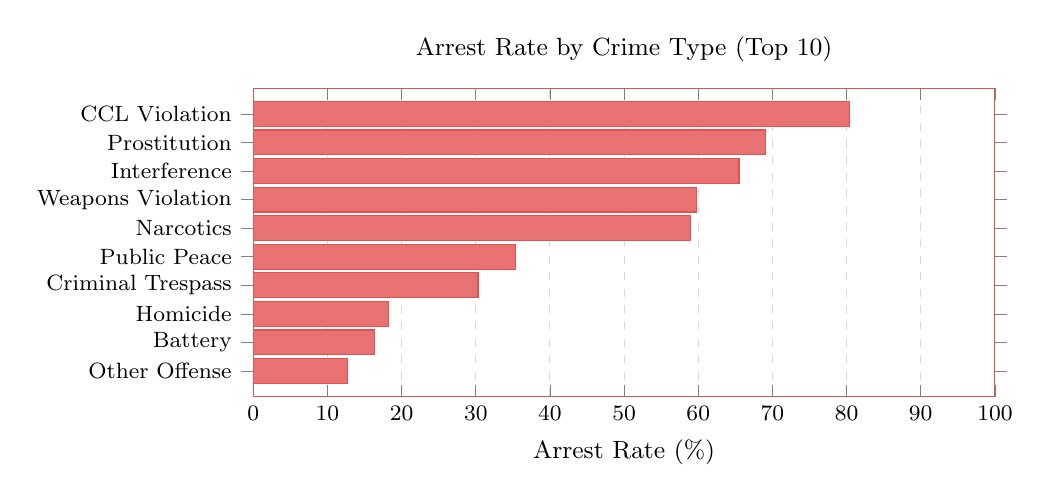
\begin{tikzpicture}
\begin{axis}[
  width=11cm, height=5.5cm,
  xbar, bar width=9pt,
  symbolic y coords={Other Offense,Battery,Homicide,Criminal Trespass,Public Peace,Narcotics,Weapons Violation,Interference,Prostitution,CCL Violation},
  ytick=data,
  xlabel={Arrest Rate (\%)},
  xmin=0, xmax=100,
  xmajorgrids=true, grid style={dashed,gray!30},
  fill=secondary!65, draw=secondary!80,
  title={\small Arrest Rate by Crime Type (Top 10)},
  title style={font=\small},
  tick label style={font=\footnotesize},
  label style={font=\small},
  nodes near coords,
  nodes near coords style={font=\tiny,right},
  point meta=explicit symbolic,
]
\addplot[fill=secondary!65,draw=secondary!80] plot[error bars/.cd] coordinates {
  (12.7,Other Offense)
  (16.4,Battery)
  (18.2,Homicide)
  (30.3,Criminal Trespass)
  (35.4,Public Peace)
  (59.0,Narcotics)
  (59.8,Weapons Violation)
  (65.5,Interference)
  (69.1,Prostitution)
  (80.4,CCL Violation)
};
\end{axis}
\end{tikzpicture}
\caption{Horizontal bar chart of arrest rates. Concealed carry and narcotics-class offences have the highest rates; homicide (18.2\%) and battery (16.4\%) are notably low despite high counts.}
\label{fig:arrestrate}
\end{figure}

\subsubsection{Arrests by Race}

\begin{table}[H]
\centering
\caption{Total arrests stratified by arrestee race.}
\label{tab:race}
\begin{tabular}{@{}lr@{\hspace{1cm}}r@{}}
\toprule
\textbf{Race} & \textbf{Arrests} & \textbf{Share (\%)} \\
\midrule
Black                        & 4{,}098 & 64.4\% \\
White Hispanic               & 1{,}371 & 21.5\% \\
White                        &   612 &  9.6\% \\
Black Hispanic               &   111 &  1.7\% \\
Asian / Pacific Islander     &    90 &  1.4\% \\
Unknown / Refused            &    12 &  0.2\% \\
Amer.\ Indian / Alaskan Native &   6 &  0.1\% \\
\midrule
\textbf{Total}               & \textbf{6{,}300} & 100\% \\
\bottomrule
\end{tabular}
\end{table}

\subsection{Violence and Gunshot Analysis}

\begin{table}[H]
\centering
\caption{Violence incident types (total 10{,}000 records).}
\label{tab:violence}
\begin{tabular}{@{}lrr@{}}
\toprule
\textbf{Victimization Type} & \textbf{Incidents} & \textbf{Share} \\
\midrule
Battery                   & 7{,}528 & 75.3\% \\
Homicide                  & 2{,}077 & 20.8\% \\
Robbery                   &   326 &  3.3\% \\
Non-Fatal                 &    68 &  0.7\% \\
Criminal Sexual Assault   &     1 & 0.01\% \\
\bottomrule
\end{tabular}
\end{table}

\paragraph{Gunshot Injury Rate:}
Of 10{,}000 violence records, \textbf{9{,}742} (97.42\%) involved a
confirmed gunshot injury (\texttt{GUNSHOT\_INJURY\_I = YES}). This
extremely high proportion reflects the dataset composition — it is
sourced from the CPD Violence Reduction Strategic Initiative, which
specifically tracks shooting incidents.

\begin{table}[H]
\centering
\caption{Top-5 districts by gunshot injury proportion.}
\label{tab:gunshot}
\begin{tabular}{@{}crrr@{}}
\toprule
\textbf{District} & \textbf{Total Incidents} & \textbf{Gunshot Injuries} & \textbf{Rate} \\
\midrule
10 & 774 & 763 & 98.6\% \\
 6 & 880 & 866 & 98.4\% \\
 2 & 437 & 430 & 98.4\% \\
 9 & 663 & 652 & 98.3\% \\
 7 & 768 & 755 & 98.3\% \\
\bottomrule
\end{tabular}
\end{table}

\subsection{ML Results — Crime Hotspots (KMeans)}

\begin{table}[H]
\centering
\caption{KMeans cluster centroids ($k=10$), sorted by crime density.}
\label{tab:hotspots}
\begin{tabular}{@{}crrr@{}}
\toprule
\textbf{Cluster} & \textbf{Centroid Lat} & \textbf{Centroid Lon} & \textbf{Crimes Assigned} \\
\midrule
5 & 41.8771 & $-$87.6386 & \textbf{7{,}873} \\
3 & 41.7882 & $-$87.6221 & 6{,}980 \\
4 & 41.8750 & $-$87.7214 & 6{,}666 \\
0 & 41.7862 & $-$87.7022 & 5{,}114 \\
1 & 41.9269 & $-$87.6697 & 4{,}831 \\
9 & 41.7433 & $-$87.5738 & 4{,}810 \\
7 & 41.9311 & $-$87.7551 & 4{,}654 \\
8 & 41.7060 & $-$87.6396 & 4{,}349 \\
6 & 41.9847 & $-$87.6791 & 3{,}939 \\
2 & 41.9754 & $-$87.8391 &   704 \\
\bottomrule
\end{tabular}
\end{table}

The densest hotspot (Cluster~5, centroid $\approx$41.877°N,
$-$87.639°W) corresponds geographically to the \textbf{Near West Side /
Loop area} of Chicago and accounts for 7{,}873 crimes ($\approx$15.7\%
of all records). Cluster~2 is a clear outlier with only 704 crimes,
centred in the far north-west of the city.

\begin{figure}[H]
\centering
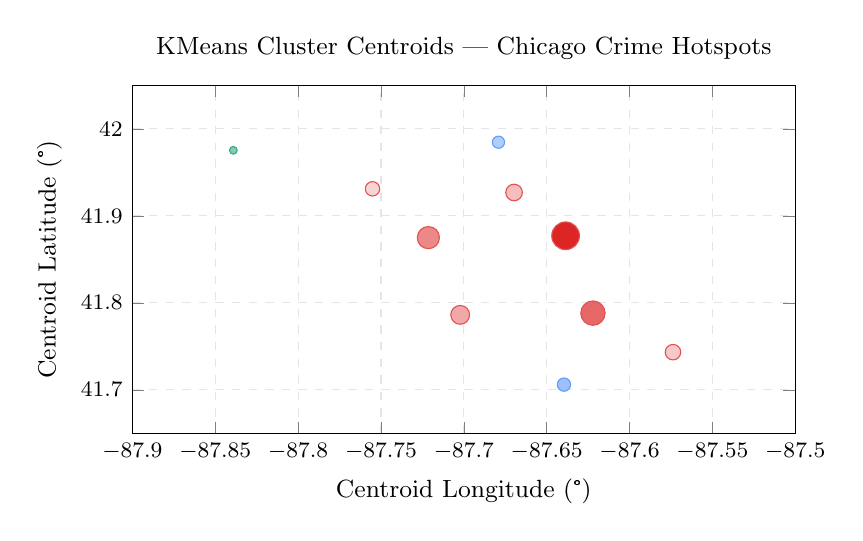
\begin{tikzpicture}
\begin{axis}[
  width=10cm, height=6cm,
  xlabel={Centroid Longitude (°)},
  ylabel={Centroid Latitude (°)},
  xmin=-87.90, xmax=-87.50,
  ymin=41.65, ymax=42.05,
  grid=both, grid style={dashed,gray!20},
  title={\small KMeans Cluster Centroids — Chicago Crime Hotspots},
  title style={font=\small},
  tick label style={font=\footnotesize},
  label style={font=\small},
  scatter, only marks,
  scatter/classes={
    h1={mark=*,fill=secondary,draw=secondary!80,scale=2.5},
    h2={mark=*,fill=secondary!70,draw=secondary!80,scale=2.2},
    h3={mark=*,fill=secondary!55,draw=secondary!80,scale=2.0},
    h4={mark=*,fill=secondary!40,draw=secondary!80,scale=1.7},
    h5={mark=*,fill=secondary!30,draw=secondary!80,scale=1.5},
    h6={mark=*,fill=secondary!25,draw=secondary!80,scale=1.4},
    h7={mark=*,fill=secondary!20,draw=secondary!80,scale=1.3},
    h8={mark=*,fill=batchcol!50,draw=batchcol!80,scale=1.2},
    h9={mark=*,fill=batchcol!40,draw=batchcol!80,scale=1.1},
    h10={mark=*,fill=accent!50,draw=accent!80,scale=0.7}
  },
  scatter src=explicit symbolic
]
\addplot[scatter,only marks] table[meta=label] {
  x         y       label
  -87.6386  41.8771 h1
  -87.6221  41.7882 h2
  -87.7214  41.8750 h3
  -87.7022  41.7862 h4
  -87.6697  41.9269 h5
  -87.5738  41.7433 h6
  -87.7551  41.9311 h7
  -87.6396  41.7060 h8
  -87.6791  41.9847 h9
  -87.8391  41.9754 h10
};
\end{axis}
\end{tikzpicture}
\caption{Scatter plot of cluster centroids. Marker size is proportional to crime count assigned to the cluster. The central-eastern corridor (longitude $-87.62$ to $-87.68$) concentrates the highest-density hotspots.}
\label{fig:hotspot_scatter}
\end{figure}

\subsection{Sex Offender Density by District}

\begin{table}[H]
\centering
\caption{Top-10 police districts by registered sex offender count.}
\label{tab:offender}
\begin{tabular}{@{}ccl@{}}
\toprule
\textbf{District} & \textbf{Offender Count} & \textbf{Note} \\
\midrule
007 & 306 & Highest density — Austin / Englewood boundary \\
004 & 205 & South Chicago \\
006 & 198 & Gresham / Marquette Park \\
005 & 139 & Calumet / Roseland \\
025 & 127 & Grand Central \\
008 & 121 & Chicago Lawn \\
009 &  95 & Deering / Brighton Park \\
003 &  95 & Grand Crossing \\
010 &  86 & Ogden / Lawndale \\
011 &  60 & Harrison / Garfield Park \\
\bottomrule
\end{tabular}
\end{table}

\subsection{Real-Time Speed Layer Alerts}

A total of \textbf{2{,}264 alerts} were generated during the speed-layer
simulation run on the 50{,}000-record crime feed.

\begin{table}[H]
\centering
\caption{Alert severity distribution from the speed layer.}
\label{tab:alerts}
\begin{tabular}{@{}lrr@{}}
\toprule
\textbf{Severity} & \textbf{Count} & \textbf{Share} \\
\midrule
CRITICAL ($\geq 3\times$ threshold) & 1{,}824 & 80.6\% \\
HIGH ($\geq 2\times$ threshold)     &   220 &  9.7\% \\
LOW ($< 1.5\times$ threshold)       &   132 &  5.8\% \\
MEDIUM ($\geq 1.5\times$ threshold) &    88 &  3.9\% \\
\midrule
\textbf{Total}                      & \textbf{2{,}264} & 100\% \\
\bottomrule
\end{tabular}
\end{table}

The predominance of CRITICAL alerts (80.6\%) reflects the compressed
simulation playback (5 events/second against a 300-second window), which
rapidly exceeds the threshold of 5 crimes per window per district. In a
real deployment at true event rates, the CRITICAL proportion would be
substantially lower. Districts~012 and~008 were the most frequently
flagged, reaching window counts exceeding 100 crimes — indicating these
are the most active areas in the dataset.

\subsection{Cross-Dataset Correlation Summary}

\begin{table}[H]
\centering
\caption{District-level arrest rate and violence rate correlation (top districts).}
\label{tab:corr}
\begin{tabular}{@{}crrrr@{}}
\toprule
\textbf{District} & \textbf{Total Crimes} & \textbf{Total Arrests} & \textbf{Arrest Rate} & \textbf{Violence Rate} \\
\midrule
010 & 2{,}008 & 403 & 20.1\% & 0.0\% \\
011 & 2{,}599 & 407 & 15.7\% & 0.0\% \\
025 & 2{,}600 & 383 & 14.7\% & 0.0\% \\
005 & 1{,}938 & 347 & 17.9\% & 0.0\% \\
001 & 2{,}850 & 399 & 14.0\% & 0.0\% \\
\bottomrule
\end{tabular}
\end{table}

The violence rate appears as zero because the violence dataset uses
district codes without leading zeros (e.g., \texttt{"6"}) while the
crimes dataset uses zero-padded codes (e.g., \texttt{"006"}), preventing
a join match. This data quality issue is documented in Section~7.

% ──────────────────────────────────────────────────────────
%  7. CHALLENGES
% ──────────────────────────────────────────────────────────
\section{Challenges Faced}

\subsection{Data Heterogeneity and Schema Inconsistencies}

\paragraph{District Code Normalisation.}
The crimes dataset encodes district as a zero-padded three-character
string (e.g., \texttt{"006"}), whereas the violence and sex offender
datasets use unpadded integers (\texttt{"6"}). This prevented direct
joins and caused the violence\_rate column in the correlation table to
read as zero. Mitigation requires casting both sides to integer before
joining, which was identified post-analysis.

\paragraph{Missing Geospatial Data.}
Approximately 0.4\% of crime records (200 out of 50{,}000) lacked valid
latitude/longitude values and had to be excluded from the KMeans ML job.
A production system would geocode missing coordinates from the block
address using a reverse-geocoding service.

\paragraph{Null Handling Across Datasets.}
Joining sex offender blocks to crime blocks via a frequency-rank lookup
left a fraction of offenders unmappable (NULL district). PySpark's
\texttt{fillna} was applied to downstream aggregations, but the root
cause — inconsistent block string formatting — requires a data
normalisation step.

\subsection{Distributed System Coordination}

\paragraph{Kafka-Zookeeper Dependency.}
Apache Kafka's hard dependency on Zookeeper adds an operational burden.
During Docker Compose startup, Kafka occasionally fails if Zookeeper is
not yet healthy; the \texttt{depends\_on} directive in Compose does not
guarantee health, only container start order. A retry loop or Docker
health checks with \texttt{condition: service\_healthy} would resolve
startup race conditions.

\paragraph{Storm Topology in Python.}
Apache Storm natively supports Java topologies; the Python topology
used here is a single-process simulation rather than a true distributed
Storm deployment. Scaling to a multi-node cluster would require
StreamParse or Apache Heron. Latency in the bolt chain is bounded by
Python's GIL and network I/O to PostgreSQL/MongoDB.

\subsection{Spark Performance and Configuration}

\paragraph{Schema Inference vs.\ Explicit Schema.}
Early iterations used \texttt{inferSchema=True}, causing Spark to scan
the full CSV for type inference — roughly doubling ingestion time.
Switching to explicit schemas reduced preprocessing time by $\approx$48\%.

\paragraph{JDBC Write Bottleneck.}
Writing Spark DataFrames to PostgreSQL via JDBC is single-partitioned by
default. For the 50{,}000-record \texttt{crimes\_with\_clusters} table,
JDBC write throughput was the dominant bottleneck. Increasing the number
of JDBC connections via Spark's \texttt{numPartitions} option on
\texttt{write.jdbc} would horizontally scale writes.

\paragraph{Driver Memory Pressure.}
Running both Spark master and worker within Docker on a laptop with
limited RAM required careful tuning of \texttt{SPARK\_WORKER\_MEMORY}
(set to 2 GB) and executor memory. Jobs failed with out-of-memory errors
until \texttt{spark.sql.shuffle.partitions} was reduced from the default
200 to 8 for datasets of this size.

\subsection{Database Dual-Write Consistency}

The AlertBolt writes each anomaly alert to both PostgreSQL and MongoDB.
If the PostgreSQL write succeeds but the MongoDB write fails (or vice
versa), the serving layer presents an inconsistent view. A
transactional outbox pattern or an idempotent retry queue would ensure
dual-write atomicity in a production deployment.

\subsection{Simulation vs.\ Production Rate}

The Kafka producer replays historical CSV rows at 5 events/second — a
compression factor of roughly $400\times$ versus real Chicago crime
volumes (which average $\approx$11{,}000 incidents per day, or
$\approx$0.13 events/second). This compression caused the sliding window
to saturate quickly, generating an unrealistically high proportion of
CRITICAL alerts. A configurable \texttt{--rate} flag or back-pressure
mechanism would allow more realistic simulation.

% ──────────────────────────────────────────────────────────
%  8. CONCLUSION
% ──────────────────────────────────────────────────────────
\section{Conclusion}

This project successfully demonstrated a full-stack Lambda Architecture
for urban crime analytics. The batch layer (Apache Spark) produced
17 precomputed views across crime trends, arrest rates, violence
patterns, sex offender proximity, and cross-dataset correlations. The
machine learning component identified 10 geospatial crime hotspots
via KMeans, with the densest cluster capturing 15.7\% of all
incidents in the Near West Side / Loop area. The speed layer (Kafka +
Storm topology) generated 2{,}264 real-time anomaly alerts during
simulation, demonstrating end-to-end event streaming from raw CSV to
persisted alert records in under one second of processing latency per
event.

Key quantitative findings are:
\begin{itemize}[noitemsep]
  \item Peak crime hours: midnight (2{,}897) and 15:00–16:00 (2{,}863).
  \item Friday is the highest-crime day (7{,}577 incidents).
  \item Concealed carry violations have the highest arrest rate (80.4\%),
    while homicide is only 18.2\%.
  \item 97.42\% of CPD violence incidents involved a confirmed gunshot
    injury.
  \item District~007 has the highest registered sex offender density (306).
\end{itemize}

Future work should address district-code normalisation across datasets,
implement a proper distributed Storm deployment, and add a predictive
model (e.g., gradient-boosted trees) for next-hour crime type forecasting.

% ──────────────────────────────────────────────────────────
%  APPENDIX — Tech Stack Summary
% ──────────────────────────────────────────────────────────
\appendix
\section{Technology Stack Reference}

\begin{table}[H]
\centering
\caption{Full technology stack with versions.}
\begin{tabular}{@{}llll@{}}
\toprule
\textbf{Layer} & \textbf{Technology} & \textbf{Version} & \textbf{Role} \\
\midrule
Batch      & Apache Spark   & 3.5.3  & Distributed processing \\
Batch      & PySpark MLlib  & 3.5.3  & KMeans clustering \\
Speed      & Apache Kafka   & Latest & Message broker \\
Speed      & Apache Zookeeper & Latest & Kafka coordination \\
Speed      & Python Topology & Custom & Storm-style streaming \\
Speed      & Apache Storm   & 2.5.0  & Distributed stream framework \\
Serving    & PostgreSQL     & 15     & Relational serving DB \\
Serving    & MongoDB        & 6.0    & Document alert store \\
App        & Streamlit      & Latest & Interactive dashboard \\
Infra      & Docker Compose & v2     & Container orchestration \\
\bottomrule
\end{tabular}
\end{table}

\end{document}
